\documentclass[12pt]{article}

\title{MIT 18-S-S996: Category theory for scientists, Spring 2013  \\ Homework and personal notes}
\author{Armand Sumo -- \texttt{armandsumo@gmail.com}}
\usepackage{etex}
\usepackage{savesym}
\usepackage{amssymb, amsmath,amsthm,amscd}
%\savesymbol{lrcorner}
\usepackage{txfonts}
%\usepackage{marvosym}
\usepackage{wasysym}
\savesymbol{Sun}\savesymbol{Mercury}\savesymbol{Venus}\savesymbol{Earth}\savesymbol{Mars}\savesymbol{Jupiter}\savesymbol{Saturn}\savesymbol{Uranus}\savesymbol{Neptune}\savesymbol{Pluto}\savesymbol{leftmoon}\savesymbol{rightmoon}\savesymbol{fullmoon}\savesymbol{newmoon}\savesymbol{Aries}\savesymbol{Taurus}\savesymbol{Gemini}\savesymbol{Leo}\savesymbol{Libra}\savesymbol{Scorpio}\savesymbol{diameter}
\usepackage{mathabx}
%\usepackage{stmaryrd}
\usepackage{setspace}
\usepackage{chngcntr}
\usepackage[tt]{titlepic}
\usepackage{enumerate,makecell}
\usepackage{makeidx,tabularx,dashbox}
\usepackage[usenames,dvipsnames]{xcolor}
\usepackage[bookmarks=true,colorlinks=true, linkcolor=MidnightBlue, citecolor=cyan]{hyperref}
\usepackage{lmodern}
\usepackage{graphicx,float}
\usepackage{multirow}
\usepackage{geometry}
\newgeometry{left=1.6in,right=1.6in,top=1.4in,bottom=1.4in}

\usepackage{color}
\usepackage[all,poly,color,matrix,arrow]{xy}
\makeindex

%\usepackage{showkeys}

\newcommand{\comment}[1]{}

\newcommand{\longnote}[2][4.9in]{\fcolorbox{black}{yellow}{\parbox{#1}{\color{black} #2}}}
\newcommand{\shortnote}[1]{\fcolorbox{black}{yellow}{\color{black} #1}}
\newcommand{\start}[1]{\shortnote{Start here: #1.}}
\newcommand{\q}[1]{\begin{question}#1\end{question}}
\newcommand{\g}[1]{\begin{guess}#1\end{guess}}
\newcommand{\cfbox}[2]{
    \colorlet{currentcolor}{.}
    {\color{#1}
    \fbox{\color{currentcolor}#2}}
}

\def\tn{\textnormal}
\def\mf{\mathfrak}
\def\mc{\mathcal}
\newcommand{\qt}[1]{\tn{``}#1\tn{"}}

\def\ZZ{{\mathbb Z}}
\def\QQ{{\mathbb Q}}
\def\RR{{\mathbb R}}
\def\CC{{\mathbb C}}
\def\AA{{\mathbb A}}
\def\PP{{\mathbb P}}
\def\NN{{\mathbb N}}


\def\Hom{\tn{Hom}}
\def\Path{\tn{Path}}
\def\Paths{\tn{Paths}}
\def\List{\tn{List}}
\def\im{\tn{im}}
\def\Fun{\tn{Fun}}
\def\Ob{\tn{Ob}}
\def\Skel{\tn{Skel}}
\def\Op{\tn{Op}}
\def\PK{\tn{PK}}
\def\FK{\tn{FK}}
\def\SEL*{\tn{SEL*}}
\def\Res{\tn{Res}}
\def\hsp{\hspace{.3in}}
\newcommand{\hsps}[1]{{\hspace{2mm} #1\hspace{2mm}}}
\newcommand{\tin}[1]{\text{\tiny #1}}

\def\singleton{\{\smiley\}}
\newcommand{\boxtitle}[1]{\begin{center}#1\end{center}\vspace{-.1in}}
\newcommand{\singlefun}[1]{\star^{#1}}
\newcommand{\pullb}[1]{\Delta_{#1}}
\newcommand{\lpush}[1]{\Sigma_{#1}}
\newcommand{\rpush}[1]{\Pi_{#1}}
\def\lcone{^\triangleleft}
\def\rcone{^\triangleright}
\def\to{\rightarrow}
\def\from{\leftarrow}
\def\down{\downarrrow}
\def\Down{\Downarrow}
\def\cross{\times}
\def\taking{\colon}
\def\inj{\hookrightarrow}
\def\surj{\twoheadrightarrow}
\def\too{\longrightarrow}
\newcommand{\xyright}[1]{\xymatrix{~\ar[r]#1&}}
\newcommand{\xydown}[1]{\xymatrix{~\ar[d]#1\\~}}
\newcommand{\xydoown}[1]{\xymatrix{~\ar[ddd]#1\\\parbox{0in}{~}\\\parbox{0in}{~}\\~}}
\def\fromm{\longleftarrow}
\def\tooo{\longlongrightarrow}
\def\tto{\rightrightarrows}
\def\ttto{\equiv\!\!>}
\def\ss{\subseteq}
\def\superset{\supseteq}
\def\iso{\cong}
\def\down{\downarrow}
\def\|{{\;|\;}}
\def\m1{{-1}}
\def\op{^\tn{op}}
\def\loc{\tn{loc}}
\def\la{\langle}
\def\ra{\rangle}
\def\wt{\widetilde}
\def\wh{\widehat}
\def\we{\simeq}
\def\ol{\overline}
\def\ul{\underline}
\def\plpl{+\!\!+\hspace{1pt}}
\def\acts{\lefttorightarrow}
\def\vect{\overrightarrow}
\def\qeq{\mathop{=}^?}
\def\del{\partial\,}

\def\rr{\raggedright}

%\newcommand{\LMO}[1]{\bullet^{#1}}
%\newcommand{\LTO}[1]{\bullet^{\tn{#1}}}
\newcommand{\LMO}[1]{\stackrel{#1}{\bullet}}
\newcommand{\LTO}[1]{\stackrel{\tt{#1}}{\bullet}}
\newcommand{\LA}[2]{\ar[#1]^-{\tn {#2}}}
\newcommand{\LAL}[2]{\ar[#1]_-{\tn {#2}}}
\newcommand{\obox}[3]{\stackrel{#1}{\fbox{\parbox{#2}{#3}}}}
\newcommand{\labox}[2]{\obox{#1}{1.6in}{#2}}
\newcommand{\mebox}[2]{\obox{#1}{1in}{#2}}
\newcommand{\smbox}[2]{\stackrel{#1}{\fbox{#2}}}
\newcommand{\fakebox}[1]{\tn{$\ulcorner$#1$\urcorner$}}
\newcommand{\sq}[4]{\xymatrix{#1\ar[r]\ar[d]&#2\ar[d]\\#3\ar[r]&#4}}
\newcommand{\namecat}[1]{\begin{center}$#1:=$\end{center}}

\def\monOb{\blacktriangle}

\def\ullimit{\ar@{}[rd]|(.25)*+{\Large\lrcorner}}
\def\urlimit{\ar@{}[ld]|(.25)*+{\Large\llcorner}}
\def\lllimit{\ar@{}[ru]|(.25)*+{\Large\urcorner}}
\def\lrlimit{\ar@{}[lu]|(.25)*+{\Large\ulcorner}}
\def\ulhlimit{\ar@{}[rd]|(.3)*+{\diamond}}
\def\urhlimit{\ar@{}[ld]|(.3)*+{\diamond}}
\def\llhlimit{\ar@{}[ru]|(.3)*+{\diamond}}
\def\lrhlimit{\ar@{}[lu]|(.3)*+{\diamond}}
\newcommand{\clabel}[1]{\ar@{}[rd]|(.5)*+{#1}}
\newcommand{\TriRight}[7]{\xymatrix{#1\ar[dr]_{#2}\ar[rr]^{#3}&&#4\ar[dl]^{#5}\\&#6\ar@{}[u] |{\Longrightarrow}\ar@{}[u]|>>>>{#7}}}
\newcommand{\TriLeft}[7]{\xymatrix{#1\ar[dr]_{#2}\ar[rr]^{#3}&&#4\ar[dl]^{#5}\\&#6\ar@{}[u] |{\Longleftarrow}\ar@{}[u]|>>>>{#7}}}
\newcommand{\TriIso}[7]{\xymatrix{#1\ar[dr]_{#2}\ar[rr]^{#3}&&#4\ar[dl]^{#5}\\&#6\ar@{}[u] |{\Longleftrightarrow}\ar@{}[u]|>>>>{#7}}}


\newcommand{\arr}[1]{\ar@<.5ex>[#1]\ar@<-.5ex>[#1]}
\newcommand{\arrr}[1]{\ar@<.7ex>[#1]\ar@<0ex>[#1]\ar@<-.7ex>[#1]}
\newcommand{\arrrr}[1]{\ar@<.9ex>[#1]\ar@<.3ex>[#1]\ar@<-.3ex>[#1]\ar@<-.9ex>[#1]}
\newcommand{\arrrrr}[1]{\ar@<1ex>[#1]\ar@<.5ex>[#1]\ar[#1]\ar@<-.5ex>[#1]\ar@<-1ex>[#1]}

\newcommand{\To}[1]{\xrightarrow{#1}}
\newcommand{\Too}[1]{\xrightarrow{\ \ #1\ \ }}
\newcommand{\From}[1]{\xleftarrow{#1}}
\newcommand{\Fromm}[1]{\xleftarrow{\ \ #1\ \ }}

\newcommand{\Adjoint}[4]{\xymatrix@1{#2 \ar@<.5ex>[r]^-{#1} & #3 \ar@<.5ex>[l]^-{#4}}}
\newcommand{\adjoint}[4]{\xymatrix{#1\taking #2\ar@<.5ex>[r]& #3\hspace{1pt}:\hspace{-2pt} #4\ar@<.5ex>[l]}}

\def\id{\tn{id}}
\def\Top{{\bf Top}}
\def\Cat{{\bf Cat}}
\def\Oprd{{\bf Oprd}}
\def\Str{{\bf Str}}
\def\Mon{{\bf Mon}}
\def\Grp{{\bf Grp}}
\def\Grph{{\bf Grph}}
\def\Type{{\bf Type}}
\def\Supp{{\bf Supp}}
\def\Dist{{\bf Dist}}
\def\Vect{{\bf Vect}}
\def\Kls{{\bf Kls}}
\def\Prop{{\bf Prop}}
\def\FLin{{\bf FLin}}
\def\Set{{\bf Set}}
\def\Sets{{\bf Sets}}
\def\PrO{{\bf PrO}}
\def\Star{{\bf Star}}
\def\Cob{{\bf Cob}}
\def\Qry{{\bf Qry}}
\def\set{{\text \textendash}{\bf Set}}
\def\sSet{{\bf sSet}}
\def\sSets{{\bf sSets}}
\def\Grpd{{\bf Grpd}}
\def\Pre{{\bf Pre}}
\def\Shv{{\bf Shv}}
\def\Rings{{\bf Rings}}
\def\bD{{\bf \Delta}}
\def\dispInt{\parbox{.1in}{$\int$}}
\def\bhline{\Xhline{2\arrayrulewidth}}
\def\bbhline{\Xhline{2.5\arrayrulewidth}}
\def\bbbhline{\Xhline{3\arrayrulewidth}}


\def\colim{\mathop{\tn{colim}}}
\def\hocolim{\mathop{\tn{hocolim}}}

\def\mcA{\mc{A}}
\def\mcB{\mc{B}}
\def\mcC{\mc{C}}
\def\mcD{\mc{D}}
\def\mcE{\mc{E}}
\def\mcF{\mc{F}}
\def\mcG{\mc{G}}
\def\mcH{\mc{H}}
\def\mcI{\mc{I}}
\def\mcJ{\mc{J}}
\def\mcK{\mc{K}}
\def\mcL{\mc{L}}
\def\mcM{\mc{M}}
\def\mcN{\mc{N}}
\def\mcO{\mc{O}}
\def\mcP{\mc{P}}
\def\mcQ{\mc{Q}}
\def\mcR{\mc{R}}
\def\mcS{\mc{S}}
\def\mcT{\mc{T}}
\def\mcU{\mc{U}}
\def\mcV{\mc{V}}
\def\mcW{\mc{W}}
\def\mcX{\mc{X}}
\def\mcY{\mc{Y}}
\def\mcZ{\mc{Z}}

\def\undsc{\rule{2mm}{0.4pt}}
\def\Loop{{\mcL oop}}
\def\LoopSchema{{\parbox{.5in}{\fbox{\xymatrix{\LMO{s}\ar@(l,u)[]^f}}}}}

\newtheorem{theorem}[subsubsection]{Theorem}
\newtheorem{lemma}[subsubsection]{Lemma}
\newtheorem{proposition}[subsubsection]{Proposition}
\newtheorem{corollary}[subsubsection]{Corollary}
\newtheorem{fact}[subsubsection]{Fact}

\theoremstyle{remark}
\newtheorem{remark}[subsubsection]{Remark}
\newtheorem{example}[subsubsection]{Example}
\newtheorem{warning}[subsubsection]{Warning}
\newtheorem{question}[subsubsection]{Question}
\newtheorem{guess}[subsubsection]{Guess}
\newtheorem{answer}[subsubsection]{Answer}
\newtheorem{construction}[subsubsection]{Construction}
\newtheorem{rules}[subsubsection]{Rules of good practice}
\newtheorem{exc}[subsubsection]{Exercise}
%\newenvironment{exercise}{\begin{exc}}{\hspace*{\fill}$\lozenge$\end{exc}}
\newtheorem{app}[subsubsection]{Application}
\newenvironment{application}{\begin{app}}{\hspace*{\fill}$\lozenge\lozenge$\end{app}}

%\newenvironment{exercise}{\addtocounter{theorem}{1}\vspace{.1in}\begin{sloppypar}\noindent{\em Exercise}\;\arabic{chapter}.\arabic{section}.\arabic{subsection}.\arabic{theorem}.}{\end{sloppypar}\vspace{.1in}}

\newenvironment{slogan}{\addtocounter{subsubsection}{1}\vspace{.1in}\begin{sloppypar}\noindent{\em Slogan}\;\arabic{chapter}.\arabic{section}.\arabic{subsection}.\arabic{subsubsection}. \begin{quote}``\slshape}{"\end{quote}\end{sloppypar}\vspace{.1in}}

%\newenvironment{application}{\addtocounter{subsubsection}{1}\vspace{.1in}\begin{sloppypar}\noindent{\em Application}\;\arabic{chapter}.\arabic{section}.\arabic{subsection}.\arabic{subsubsection}. \begin{quote}}{\end{quote}\end{sloppypar}\vspace{.1in}}
\makeatletter\let\c@figure\c@equation\makeatother

\theoremstyle{definition}
\newtheorem{definition}[subsubsection]{Definition}
\newtheorem{notation}[subsubsection]{Notation}
\newtheorem{conjecture}[subsubsection]{Conjecture}
\newtheorem{postulate}[subsubsection]{Postulate}


%\newtheorem{theorem}{Theorem}[subsection]
%\newtheorem{lemma}[theorem]{Lemma}
%\newtheorem{proposition}[theorem]{Proposition}
%\newtheorem{corollary}[theorem]{Corollary}
%\newtheorem{fact}[theorem]{Fact}
%
%\theoremstyle{remark}
%\newtheorem{remark}[theorem]{Remark}
%\newtheorem{example}[theorem]{Example}
%\newtheorem{warning}[theorem]{Warning}
%\newtheorem{question}[theorem]{Question}
%\newtheorem{guess}[theorem]{Guess}
%\newtheorem{answer}[theorem]{Answer}
%\newtheorem{construction}[theorem]{Construction}
%\newtheorem{rules}[theorem]{Rules of good practice}
%\newtheorem{exc}[theorem]{Exercise}
%%\newenvironment{exercise}{\addtocounter{theorem}{1}\vspace{.1in}\begin{sloppypar}\noindent{\em Exercise}\;\arabic{chapter}.\arabic{section}.\arabic{subsection}.\arabic{theorem}.}{\end{sloppypar}\vspace{.1in}}
%\newenvironment{exercise}{\begin{exc}}{\hspace*{\fill}$\lozenge$\end{exc}}
%
%\theoremstyle{definition}
%\newtheorem{definition}[theorem]{Definition}
%\newtheorem{notation}[theorem]{Notation}
%\newtheorem{conjecture}[theorem]{Conjecture}
%\newtheorem{postulate}[theorem]{Postulate}

\def\Finm{{\bf Fin_{m}}}
\def\Prb{{\bf Prb}}
\def\Prbs{{\wt{\bf Prb}}}
\def\El{{\bf El}}
\def\Gr{{\bf Gr}}
\def\DT{{\bf DT}}
\def\DB{{\bf DB}}
\def\Tables{{\bf Tables}}
\def\Sch{{\bf Sch}}
\def\Fin{{\bf Fin}}
\def\P{{\bf P}}
\def\SC{{\bf SC}}
\def\ND{{\bf ND}}
\def\Poset{{\bf Poset}}


\newcommand{\MainCatLarge}[1]{ 
	\stackrel{#1}{
		\parbox{4.5in}{\fbox{\parbox{4.4in}{\begin{center}\underline{{\tt Employee} manager worksIn $\simeq$ {\tt Employee} worksIn}\hsp  \underline{{\tt Department} secretary worksIn $\simeq$ {\tt Department}}\end{center}~\\\\\\
			\xymatrix@=8pt{&\LTO{Employee}\ar@<.5ex>[rrrrr]^{\tn{worksIn}}\ar@(l,u)[]+<5pt,10pt>^{\tn{manager}}\ar[dddl]_{\tn{first}}\ar[dddr]^{\tn{last}}&&&&&\LTO{Department}\ar@<.5ex>[lllll]^{\tn{secretary}}\ar[ddd]^{\tn{name}}\\\\\\\LTO{FirstNameString}&&\LTO{LastNameString}&~&~&~&\LTO{DepartmentNameString}
			}
		}}}
	}
}
%\CompileMatrices

\setcounter{secnumdepth}{4}
\setcounter{tocdepth}{1}
\usepackage{enumitem}

%\ Add Extra Level of Section
\usepackage{titlesec}

\titleformat{\paragraph}
{\normalfont\normalsize\bfseries}{\theparagraph}{1em}{}
\titlespacing*{\paragraph}
{0pt}{3.25ex plus 1ex minus .2ex}{1.5ex plus .2ex}
%change exercise notation
\usepackage{exercise}
%use fullpage
%\usepackage{fullpage}
\renewcounter{Exercise}[subsubsection]% Reset counter every chapter
%add Quiver package for Diagrams
\usepackage{quiver}

%%%%%
\begin{document}
\begin{large}
  \maketitle
  \begin{center}

  \vspace{-0.3in}
  \begin{tabular}{rl}
  Collaborators: & 
  \end{tabular}
  \end{center}

All of this is my own work.

\noindent
\rule{\linewidth}{0.4pt}
\section{Introduction}
\section{The category of sets}
\subsection{Sets and function}
\subsubsection{Sets}\label{sec:sets}
\begin{Exercise}
The set of all sets of $A=\{1,2,3\}$, also called the power set of $A$, is \begin{align*}\mathcal{P}(A)=\{\emptyset,A,1,2,3,\{1,2\},\{1,3\},\{2,3\},\{1,2,3\}\} \end{align*}
\end{Exercise}
\begin{Exercise}
\begin{enumerate}[label=(\alph*)]
\item
Because each element of the set of photo-receptive cells ($PR$) connects to exactly one element of the set of retino-ganglial cells($RG$) and no elements of $PR$ connect to two elements of $RG$,  the only valid function would be from $PR\rightarrow RG $. 
\item Each neuron forms at least one synapse with other neurons(otherwise it dies). Thus, the set of function-like connections between brain parts is a subset of the set of all biologically possible connections between brain parts.\\ It therefore seems plausible that the connection patterns that exists between other areas of the brain are function-like.
\end{enumerate}
\end{Exercise}

\begin{Exercise}
As depicted in (2.2), the elements of the codomain of $f$ that receive at least one arrows are $y_1,y_2,y_4$. Therefore $im(f)=\{y_1,y_2,y_4\}$.
\end{Exercise}
\begin{Exercise}
\begin{enumerate}[label=(\alph*)]
\item
$A=\{1,2,3,4,5\}$ and $B=\{x,y\}$. \\
Since each element in $A$ has $|B|$ choices, by the product rule, the total number of functions from $A$ to $B$ is \begin{align*}
|\text{Hom}_\text{Set}(A,B)|=\underbrace{|B|\times |B| \times \cdots \times |B|}_{\text{$|A|$ times}} = 2^5 = 32.
\end{align*}
\item Similarly, since each element of $B$ has $|A|$ choices, the total number of functions from $B$ to $A$ is \begin{align*}
|\text{Hom}_\text{Set}(B,A)|=\underbrace{|A|\times |A| \times \cdots \times |A|}_{\text{$|B|$ times}} = 5^2 = 25.
\end{align*}
\end{enumerate}
\end{Exercise}
\begin{Exercise}
\begin{enumerate}[label=(\alph*)]
\item One set $A$ such that for all sets $X$ there's exactly one element in \begin{align*}\text{Hom}_\text{Set}(X,A) \text{\ is \ } A =\emptyset
\end{align*}. 
This is because all sets contain the empty set and the empty set can only be mapped onto itself. 
\item Similarly, one set $B$ such that for all sets $X$ there's exactly one element in $\text{Hom}_\text{Set}(B,X)$ is $B = \emptyset.$
\end{enumerate}
\end{Exercise}
\begin{Exercise}
Let $X$ be a set with cardinal $n$. 
 \begin{enumerate}[label=(\alph*)]
\item The first element of $X$ can be mapped to $n$ elements of $X$, the second to $(n-1)$, and so on and the $k$-th to $(n-(k-1))$, thus there are 
\begin{align*}
n\times(n-1)\times \cdots \times 1= n!
\end{align*} isomorphisms from $X$ to itself.
\item 
By convention, $0!=1$ so the formula above holds when $n=0$ and $X=\emptyset$.
\end{enumerate}
\end{Exercise}
\begin{Exercise}
There is no one-to-one correspondence between ``types" of the elements of the sets A and B so there's no obvious choice for which element of B will be associated to each element of the codomain of $f$. For this reason isn't one particular ``canonical funcion" $A \rightarrow \{1,2,3,4,5\}$
\end{Exercise} corresponding to $f$.
\begin{Exercise}
Suppose we have found a set $A$ such that for any set $X$, there's an isomorphism of sets
\begin{align*}X \cong \text{Hom}_\text{Set}(A,X)
\end{align*}
then, the two sets must have the same cardinal:
\begin{align*}|X| = |\text{Hom}_\text{Set}(A,X)|
\end{align*}
Because $\text{Hom}_\text{Set}(A,X)$ is the set of all functions from A to X, its cardinal must be $|X|^{|A|}$, hence:
\begin{align*}
|X| = |X|^{|A|}
\end{align*}
From here we can split into 2 cases, namely $|X|<1$ \text{and} $|X|>1$.\\
If $|X|>1$, applying the logarithm to both sides gives:
\begin{align*}
\text{log}|X| &= |A|{\text{log}|X|}\\
 |A| &= 1
\end{align*}
therefore, only sets $A$ with only one element can be picked.\\
If $|X|<1$, then any set $A$ can be picked.\\
Because the desired property must hold for all sets $X$, the only valid choices for $A$ are among sets containing only one element.
\end{Exercise}
\begin{Exercise}

\begin{enumerate}[label=(\alph*)]\item
If A = \{a,b,c,d\} and $f:\underline{10}\rightarrow A = \{a,b,c,c,b,a,d,d,a,b\}$, then $f(4)=c$.
\item
$s:\underline{7}\rightarrow\mathbb{N}$ given by $s(i)=i^2$ can be written as a sequence 
\begin{align*}
s =(1,4,9,16,25,36,49).
\end{align*}
\end{enumerate}
\end{Exercise}
\begin{Exercise}
\begin{enumerate}[label=(\alph*)]
\item
$|\{5,6,7\}|=3$;
\item
$|\mathbb{N}|=\infty$;
\item 
$|\{n \in \mathbb{N} \mid n \leq 5\}| = 6.$
\end{enumerate}
\end{Exercise}
\subsection{Commutative diagrams}
\subsection{Ologs}
\begin{Exercise}
Olog that captures the parent-child relationship:\\
% https://q.uiver.app/?q=WzAsMyxbMCwxLCJcXGJveGVke1xcdGV4dHthIHBlcnNvbn19Il0sWzEsMCwiXFxib3hlZHtcXHRleHR7bm8gY2hpbGRyZW59fSJdLFsxLDIsIlxcYm94ZWR7XFx0ZXh0e2EgY2hpbGR9fSJdLFswLDEsIiAgXFx0ZXh0e21heSBoYXZlfSJdLFswLDIsIlxcdGV4dHttYXkgaGF2ZX0iLDJdXQ==
\begin{tikzcd}
	& {\boxed{\text{no children}}} \\
	{\boxed{\text{a person}}} \\
	& {\boxed{\text{a child}}}
	\arrow["{  \text{can have}}", from=2-1, to=1-2]
	\arrow["{\text{can have}}"', from=2-1, to=3-2]
\end{tikzcd}
\end{Exercise}
\begin{Exercise}
Olog for human nuclear biological families:\\
% https://q.uiver.app/?q=WzAsOSxbNSwyLCJcXGJveGVke1xcdGV4dHthIHBlcnNvbn19Il0sWzAsMCwiXFxib3hlZHtcXHRleHR7YSBtYW59fSJdLFswLDQsIlxcYm94ZWR7XFx0ZXh0e2Egd29tYW59fSJdLFszLDIsIlxcYm94ZWR7XFx0ZXh0e2EgY2hpbGR9fSJdLFsxLDIsIlxcYm94ZWR7XFx0ZXh0e2EgcGFyZW50fX0iXSxbMyw0XSxbMSwxLCJcXGNoZWNrbWFyayJdLFsxLDMsIlxcY2hlY2ttYXJrIl0sWzIsMl0sWzEsMCwiXFx0ZXh0e2lzfSJdLFsyLDAsIlxcdGV4dHtpc30iXSxbMSw0LCJcXHRleHR7aXN9Il0sWzIsNCwiXFx0ZXh0e2lzfSJdLFs0LDMsIlxcdGV4dHtoYXMgYX0iXSxbMywwLCJcXHRleHR7aXN9Il1d
\begin{tikzcd}
	{\boxed{\text{a man}}} \\
	& \checkmark \\
	& {\boxed{\text{a parent}}} & {} & {\boxed{\text{a child}}} && {\boxed{\text{a person}}} \\
	& \checkmark \\
	{\boxed{\text{a woman}}} &&& {}
	\arrow["{\text{is}}", from=1-1, to=3-6]
	\arrow["{\text{is}}", from=5-1, to=3-6]
	\arrow["{\text{is}}", from=1-1, to=3-2]
	\arrow["{\text{is}}", from=5-1, to=3-2]
	\arrow["{\text{has a}}", from=3-2, to=3-4]
	\arrow["{\text{is}}", from=3-4, to=3-6]
\end{tikzcd}
\end{Exercise}
\begin{Exercise}
Given x, an operational land-line phone, consider the following. We know that $x$ is an operational land-line phone,\\
which is assigned to a phone number, which has an area code, which corresponds to a region\\
that we'll call $P(x)$.\\
We also know that $x$ is an operational land-line phone,
which is a physical phone, which is currently located in a region\\
that we'll call $Q(x)$.\\
Fact: whenever $x$ is an operational land-line phone, we will have $P(x)=Q(x)$.\\ 
\end{Exercise}
\begin{Exercise}
If the box  ``an operational land-line phone" was replaced with the box ``an operational mobile phone", the region in which it is currently located would not not always match the region corresponding to the mobile phone's phone number's area code and diagram would not commute.
\end{Exercise}
\begin{Exercise}
\begin{enumerate}[label=(\alph*)]
\item
``a book": ``not clearly an image type"\\
\item
``a material that has been fabricated by a process of type T."
\[f: \text{material} \rightarrow \text{material} \\ 
\text{ : ``has been fabricated by a process of type T"}\]
\item ``a bicycle owner"
\[f: \text{owner} \rightarrow \text{owner} \text{ : ``owns a bicycle"}\]
\item ``a child" : not clearly an image type. 
\item ``a used book"
\[f: \text{book}  \rightarrow \text{book} \\ 
\text{ : ``is used"}\]
\item ``an inhabited residence"
\[f: \text{residence} \rightarrow \text{residence} \\ 
\text{ : ``is inhabited"}\]
\end{enumerate}
\end{Exercise}
\subsection{Products and coproducts}
\begin{Exercise}
$\{a,b,c,d\}\times\{1,2,3\}$ has $|\{a,b,c,d\}| \times |\{1,2,3\}| = 4 \times 3 =12$ items. 
\end{Exercise}
\begin{Exercise}
\begin{enumerate}
\item The following diagram commutes:
% https://q.uiver.app/?q=WzAsNSxbMCwwLCIgXFxtYXRoYmJ7Wn1cXHRpbWVzXFxtYXRoYmJ7Wn1cXHRpbWVzXFxtYXRoYmJ7Wn0iXSxbNCwwLCJcXG1hdGhiYntafVxcdGltZXNcXG1hdGhiYntafSJdLFs0LDIsIlxcbWF0aGJie1p9Il0sWzAsMiwiXFxtYXRoYmJ7Wn1cXHRpbWVzXFxtYXRoYmJ7Wn0iXSxbMiwxLCJcXGNoZWNrbWFyayJdLFswLDEsIihhLGIsYylcXG1hcHN0byhhXFxjZG90IGIsYVxcY2RvdCBjKSJdLFsxLDIsIih4LHkpXFxtYXBzdG8geCt5Il0sWzAsMywiKGEsYixjKVxcbWFwc3RvIChhK2IsYykiLDJdLFszLDIsIih4LHkpXFxtYXBzdG8geHkiLDJdXQ==
\[\begin{tikzcd}
	{ \mathbb{Z}\times\mathbb{Z}\times\mathbb{Z}} &&&& {\mathbb{Z}\times\mathbb{Z}} \\
	&& \checkmark \\
	{\mathbb{Z}\times\mathbb{Z}} &&&& {\mathbb{Z}}
	\arrow["{(a,b,c)\mapsto(a\cdot b,a\cdot c)}", from=1-1, to=1-5]
	\arrow["{(x,y)\mapsto x+y}", from=1-5, to=3-5]
	\arrow["{(a,b,c)\mapsto (a+b,c)}"', from=1-1, to=3-1]
	\arrow["{(x,y)\mapsto xy}"', from=3-1, to=3-5]
\end{tikzcd}\]
\item The following diagram doesn't commute:
% https://q.uiver.app/?q=WzAsMyxbMCwwLCJcXG1hdGhiYiB7Wn0iXSxbNCwwLCJcXG1hdGhiYntafVxcdGltZXNcXG1hdGhiYntafSJdLFs0LDIsIlxcbWF0aGJie1p9Il0sWzAsMSwieCBcXG1hcHN0byAoeCwwKSJdLFsxLDIsIihhLGIpXFxtYXBzdG8gYVxcY2RvdCBiIl0sWzAsMiwiXFx0ZXh0e2lkfV9cXG1hdGhiYntafSIsMl1d
\[\begin{tikzcd}
	{\mathbb {Z}} &&&& {\mathbb{Z}\times\mathbb{Z}} \\
	\\
	&&&& {\mathbb{Z}}
	\arrow["{x \mapsto (x,0)}", from=1-1, to=1-5]
	\arrow["{(a,b)\mapsto a\cdot b}", from=1-5, to=3-5]
	\arrow["{\text{id}_\mathbb{Z}}"', from=1-1, to=3-5]
\end{tikzcd}\]
\item
The following does:
% https://q.uiver.app/?q=WzAsNCxbMCwwLCJcXG1hdGhiYiB7Wn0iXSxbNCwwLCJcXG1hdGhiYntafVxcdGltZXNcXG1hdGhiYntafSJdLFs0LDMsIlxcbWF0aGJie1p9Il0sWzMsMSwiXFxjaGVja21hcmsiXSxbMCwxLCJ4IFxcbWFwc3RvICh4LDEpIl0sWzEsMiwiKGEsYilcXG1hcHN0byBhXFxjZG90IGIiXSxbMCwyLCJcXHRleHR7aWR9X1xcbWF0aGJie1p9IiwyXV0=
\[\begin{tikzcd}
	{\mathbb {Z}} &&&& {\mathbb{Z}\times\mathbb{Z}} \\
	&&& \checkmark \\
	\\
	&&&& {\mathbb{Z}}
	\arrow["{x \mapsto (x,1)}", from=1-1, to=1-5]
	\arrow["{(a,b)\mapsto a\cdot b}", from=1-5, to=4-5]
	\arrow["{\text{id}_\mathbb{Z}}"', from=1-1, to=4-5]
\end{tikzcd}\]
\end{enumerate}
\end{Exercise}
\begin{Exercise}
\begin{align*}
|\text{Hom}_\text{Set}(A,X)| \times |\text{Hom}_\text{Set}(A,Y)| \\
= |X|^{|A|} \times |Y|^{|A|} \\
= (|X|\times|Y|)^{|A|}\\
=|\text{Hom}_\text{Set}(A,X\times Y)|
\end{align*}
\end{Exercise}
\begin{Exercise}
\begin{enumerate}[label=(\alph*)]
\item
By the universal product rule, for any function $ f : X \times Y \mapsto X $ and a function $ g : X \times Y \mapsto Y$ there's a unique function $f \times g : X \mapsto Y \times Y \times X$. \\ 
If $\pi_1 : X \times Y \mapsto X$ and $\pi_2 : X \times Y \mapsto Y$, we can define the swap function $s: X \times Y \rightarrow Y \times X$ as $s = \pi_2 \times \pi_1$, so that the diagram below commutes: 
% https://q.uiver.app/?q=WzAsNixbMywwLCJYICBcXHRpbWVzIFkiXSxbNiwzLCJZIl0sWzAsMywiWCJdLFsxLDMsIlxcY2hlY2ttYXJrIl0sWzUsMywiXFxjaGVja21hcmsiXSxbMyw2LCJZIFxcdGltZXMgWCJdLFswLDIsIlxccGlfMSJdLFswLDEsIlxccGlfMiIsMl0sWzAsNSwicyA9IFxccGlfMiBcXHRpbWVzIFxccGlfMSIsMSx7InN0eWxlIjp7ImJvZHkiOnsibmFtZSI6ImRhc2hlZCJ9fX1dLFs1LDEsIlxccGlfMSJdLFs1LDIsIlxccGlfMiIsMl1d
% https://q.uiver.app/?q=WzAsNixbMiwwLCJYICBcXHRpbWVzIFkiXSxbNCwzLCJZIl0sWzAsMywiWCJdLFsxLDMsIlxcY2hlY2ttYXJrIl0sWzMsMywiXFxjaGVja21hcmsiXSxbMiw2LCJZIFxcdGltZXMgWCJdLFswLDIsIlxccGlfMSJdLFswLDEsIlxccGlfMiIsMl0sWzAsNSwicyA9IFxccGlfMiBcXHRpbWVzIFxccGlfMSIsMSx7InN0eWxlIjp7ImJvZHkiOnsibmFtZSI6ImRhc2hlZCJ9fX1dLFs1LDEsIlxccGlfMSJdLFs1LDIsIlxccGlfMiIsMl1d
\[\begin{tikzcd}
	&& {X  \times Y} \\
	\\
	\\
	X & \checkmark && \checkmark & Y \\
	\\
	\\
	&& {Y \times X}
	\arrow["{\pi_1}", from=1-3, to=4-1]
	\arrow["{\pi_2}"', from=1-3, to=4-5]
	\arrow["{s = \pi_2 \times \pi_1}"{description}, dashed, from=1-3, to=7-3]
	\arrow["{\pi_1}", from=7-3, to=4-5]
	\arrow["{\pi_2}"', from=7-3, to=4-1]
\end{tikzcd}\]
\item 
To show that $s$ is a isomorphism, we must find a function $t : Y \times X  \mapsto  X \times Y $ such that:\\
$t \circ s = \text{id}_{X\times Y}$ and\\
$s \circ t = \text{id}_{Y\times X}$ \\
The obvious choice is $t : Y \times X  \mapsto X \times Y$ defined as \\ $t = \pi_2 \times \pi_1$. It is obvious because for any projection $p$,  $p \circ p = \text{id}$.
\end{enumerate}
\end{Exercise}
\begin{Exercise}
Because a phone is either a cellphone or a land-line phone and not both at the same time, we can think of $\ulcorner a phone \urcorner $ as the coproduct of $\ulcorner a cellphone \urcorner $ and $\ulcorner a landline-phone \urcorner $ .
\end{Exercise}
\begin{Exercise}
\begin{align*}
\text{Hom}_{\text{Set}}(X,A) \sqcup \text{Hom}_{\text{Set}}(Y,A) = \text{Hom}_{\text{Set}}(X \sqcup Y,A)
\end{align*}
\end{Exercise}
\subsection{Finite limits in Set}
\begin{Exercise}
A photon has both the properties of a wave and the properties of a particle, therefore we can label a photon that has the properties of a wave ``W" and one that has the properties of a particle ``P" and let $C = W \sqcup P $ be the set of photons that have the properties of a wave labeled as ``W" and those that have the properties of the properties of a particle labeled as ``P".
\end{Exercise}
\begin{Exercise}
% https://q.uiver.app/?q=WzAsMTEsWzIsMCwiel8xIl0sWzIsMSwiel8yIl0sWzIsMiwiel8zIl0sWzAsMCwieF8xIl0sWzAsMSwieF8yIl0sWzAsMiwieF8zIl0sWzQsMCwieV8xIl0sWzQsMSwieV8yIl0sWzQsMiwieV8zIl0sWzIsMywiel80Il0sWzQsMywieV80Il0sWzMsMF0sWzYsMF0sWzQsMV0sWzcsMV0sWzUsMV0sWzgsOV0sWzEwLDFdXQ==
\[\begin{tikzcd}
	{x_1} && {z_1} && {y_1} \\
	{x_2} && {z_2} && {y_2} \\
	{x_3} && {z_3} && {y_3} \\
	&& {z_4} && {y_4}
	\arrow[from=1-1, to=1-3]
	\arrow[from=1-5, to=1-3]
	\arrow[from=2-1, to=2-3]
	\arrow[from=2-5, to=2-3]
	\arrow[from=3-1, to=2-3]
	\arrow[from=3-5, to=4-3]
	\arrow[from=4-5, to=2-3]
\end{tikzcd}\]
The pullback of the diagram $X \overset{f}{\longrightarrow} Z \overset{g}{\longleftarrow} Y$ presented is the subset $\{z_1\}$ of $Z$. For any other subset of $Z$, either one of the following is true:\\
\begin{itemize}
\item either $f^{-1}$ or $g^{-1}$ is not a function(ex: $f^{-1}(z_2)=x_2$ and $f^{-1}(z_2)=x_3$).\\
\item some element of the chosen subset of $Z$ is not in the domain or codomain of either $f$,$g$,$f^{-1}$ or $g^{-1}$. 
\end{itemize}
\end{Exercise}
\begin{Exercise}
We're given the diagram of functions below:
% https://q.uiver.app/?q=WzAsMyxbMCwxLCJYIl0sWzEsMSwiWiJdLFsxLDAsIlkiXSxbMCwxLCJmIiwyXSxbMiwxLCJnIl1d
\[\begin{tikzcd}
	& Y \\
	X & Z
	\arrow["f"', from=2-1, to=2-2]
	\arrow["g", from=1-2, to=2-2]
\end{tikzcd}\]
\begin{enumerate}
\item
Suppose $Y = \emptyset$, because any function whose domain is the empty set has as codomain the emptyset, the fiber product $X \times_{Z}Y$ must be the empty set. 
\item
Suppose Y is any set but Z has exactly one element, then $X \times_{Z}Y$  is a set containing at most one element.
\end{enumerate}
\end{Exercise}
\begin{Exercise}
\begin{enumerate}
\item A $\ulcorner$person whose favorite color is blue$\urcorner$ is a $\ulcorner$person$\urcorner$, not a $\ulcorner$color$\urcorner$.
\item The labels seem inappropriate because a $\ulcorner$dog whose owner is a woman$\urcorner$ is not a $\ulcorner$person$\urcorner$.
\item The labels seems inappropriate because the nature of the element of the set $\ulcorner$a good fit$\urcorner$ aren't fully specified.
\end{enumerate}
\end{Exercise}
\begin{Exercise}
% https://q.uiver.app/?q=WzAsNSxbMCwzLCJcXG92ZXJzZXR7RH17XFx0ZXh0e0ROQSBtYXRlcmlhbH19Il0sWzQsMywiXFxvdmVyc2V0e0Z9e1xcdGV4dHthIGZpbmdlcnByaW50fX0iXSxbMiw0LCJcXG92ZXJzZXR7SX17XFx0ZXh0e2FuIGlkZW50aXR5fX0iXSxbMiwwLCJEIFxcdGltZXNfRiBJXFx0ZXh0ezogYSBwYWlyIH0oZCxmKSJdLFsyLDIsIlxcb3ZlcnNldHtQfXtcXHRleHR7YSBwZXJzb259fSJdLFsxLDIsIlxcdGV4dHtkZWZpbmVzfSIsMl0sWzMsMCwiXFx0ZXh0e3lpZWxkcyBhcyB9ZCIsMix7ImN1cnZlIjoyfV0sWzMsMSwiXFx0ZXh0e3lpZWxkcyBhc30gZiIsMCx7ImN1cnZlIjotMn1dLFs0LDAsIlxcdGV4dHtoYXN9ICIsMl0sWzQsMSwiXFx0ZXh0e2hhc30iXSxbNCwzLCJcXHRleHR7Y29sbGVjdGlvbiBvZiBhIEROQSBzYW1wbGV9XFxcXCBcXHRleHR7YW5kIGEgZmluZ2VycHJpbnQgfSIsMSx7InN0eWxlIjp7ImJvZHkiOnsibmFtZSI6ImRhc2hlZCJ9fX1dLFswLDIsIlxcdGV4dHtkZWZpbmVzfSJdXQ==
\[\begin{tikzcd}
	&& {D \times_F I\text{: a pair }(d,f)} \\
	\\
	&& {\overset{P}{\text{a person}}} \\
	{\overset{D}{\text{DNA material}}} &&&& {\overset{F}{\text{a fingerprint}}} \\
	&& {\overset{I}{\text{an identity}}}
	\arrow["{\text{defines}}"', from=4-5, to=5-3]
	\arrow["{\text{yields as }d}"', curve={height=12pt}, from=1-3, to=4-1]
	\arrow["{\text{yields as} f}", curve={height=-12pt}, from=1-3, to=4-5]
	\arrow["{\text{has} }"', from=3-3, to=4-1]
	\arrow["{\text{has}}", from=3-3, to=4-5]
	\arrow["{\text{collection of a DNA sample}\\ \text{and a fingerprint }}"{description}, dashed, from=3-3, to=1-3]
	\arrow["{\text{defines}}", from=4-1, to=5-3]
\end{tikzcd}\]
\end{Exercise}



\tikzset{every picture/.style={line width=0.75pt}} %set default line width to 0.75pt        

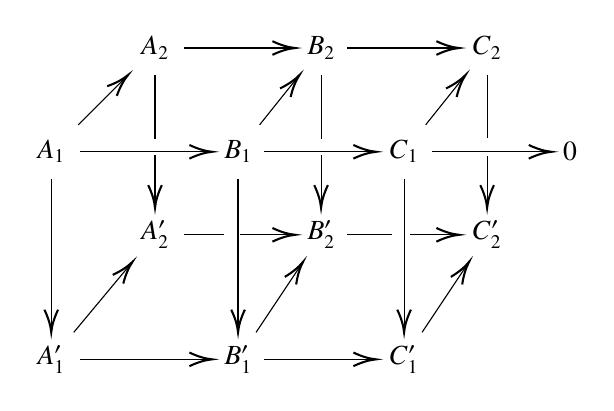
\begin{tikzpicture}[x=0.75pt,y=0.75pt,yscale=-1,xscale=1]
%uncomment if require: \path (0,235); %set diagram left start at 0, and has height of 235


% Text Node
\draw (451,71) node    {$A_{1}$};
% Text Node
\draw (501,21) node    {$A_{2}$};
% Text Node
\draw (451,171) node    {$A'_{1}$};
% Text Node
\draw (581,21) node    {$B_{2}$};
% Text Node
\draw (661,21) node    {$C_{2}$};
% Text Node
\draw (541,71) node    {$B_{1}$};
% Text Node
\draw (621,71) node    {$C_{1}$};
% Text Node
\draw (501,111) node    {$A'_{2}$};
% Text Node
\draw (581,111) node    {$B'_{2}$};
% Text Node
\draw (661,111) node    {$C'_{2}$};
% Text Node
\draw (541,171) node    {$B'_{1}$};
% Text Node
\draw (621,171) node    {$C'_{1}$};
% Text Node
\draw (701,71) node    {$0$};
% Connection
\draw    (515,21) -- (566.5,21) ;
\draw [shift={(568.5,21)}, rotate = 180] [color={rgb, 255:red, 0; green, 0; blue, 0 }  ][line width=0.75]    (10.93,-3.29) .. controls (6.95,-1.4) and (3.31,-0.3) .. (0,0) .. controls (3.31,0.3) and (6.95,1.4) .. (10.93,3.29)   ;
% Connection
\draw    (593.5,21) -- (645.5,21) ;
\draw [shift={(647.5,21)}, rotate = 180] [color={rgb, 255:red, 0; green, 0; blue, 0 }  ][line width=0.75]    (10.93,-3.29) .. controls (6.95,-1.4) and (3.31,-0.3) .. (0,0) .. controls (3.31,0.3) and (6.95,1.4) .. (10.93,3.29)   ;
% Connection
\draw    (464,58) -- (486.59,35.41) ;
\draw [shift={(488,34)}, rotate = 495] [color={rgb, 255:red, 0; green, 0; blue, 0 }  ][line width=0.75]    (10.93,-3.29) .. controls (6.95,-1.4) and (3.31,-0.3) .. (0,0) .. controls (3.31,0.3) and (6.95,1.4) .. (10.93,3.29)   ;
% Connection
\draw    (465,71) -- (526.5,71) ;
\draw [shift={(528.5,71)}, rotate = 180] [color={rgb, 255:red, 0; green, 0; blue, 0 }  ][line width=0.75]    (10.93,-3.29) .. controls (6.95,-1.4) and (3.31,-0.3) .. (0,0) .. controls (3.31,0.3) and (6.95,1.4) .. (10.93,3.29)   ;
% Connection
\draw    (553.5,71) -- (605.5,71) ;
\draw [shift={(607.5,71)}, rotate = 180] [color={rgb, 255:red, 0; green, 0; blue, 0 }  ][line width=0.75]    (10.93,-3.29) .. controls (6.95,-1.4) and (3.31,-0.3) .. (0,0) .. controls (3.31,0.3) and (6.95,1.4) .. (10.93,3.29)   ;
% Connection
\draw    (551.4,58) -- (569.35,35.56) ;
\draw [shift={(570.6,34)}, rotate = 488.66] [color={rgb, 255:red, 0; green, 0; blue, 0 }  ][line width=0.75]    (10.93,-3.29) .. controls (6.95,-1.4) and (3.31,-0.3) .. (0,0) .. controls (3.31,0.3) and (6.95,1.4) .. (10.93,3.29)   ;
% Connection
\draw    (631.4,58) -- (649.35,35.56) ;
\draw [shift={(650.6,34)}, rotate = 488.66] [color={rgb, 255:red, 0; green, 0; blue, 0 }  ][line width=0.75]    (10.93,-3.29) .. controls (6.95,-1.4) and (3.31,-0.3) .. (0,0) .. controls (3.31,0.3) and (6.95,1.4) .. (10.93,3.29)   ;
% Connection
\draw    (451,84) -- (451,156) ;
\draw [shift={(451,158)}, rotate = 270] [color={rgb, 255:red, 0; green, 0; blue, 0 }  ][line width=0.75]    (10.93,-3.29) .. controls (6.95,-1.4) and (3.31,-0.3) .. (0,0) .. controls (3.31,0.3) and (6.95,1.4) .. (10.93,3.29)   ;
% Connection
\draw    (465,171) -- (526.5,171) ;
\draw [shift={(528.5,171)}, rotate = 180] [color={rgb, 255:red, 0; green, 0; blue, 0 }  ][line width=0.75]    (10.93,-3.29) .. controls (6.95,-1.4) and (3.31,-0.3) .. (0,0) .. controls (3.31,0.3) and (6.95,1.4) .. (10.93,3.29)   ;
% Connection
\draw    (553.5,171) -- (605.5,171) ;
\draw [shift={(607.5,171)}, rotate = 180] [color={rgb, 255:red, 0; green, 0; blue, 0 }  ][line width=0.75]    (10.93,-3.29) .. controls (6.95,-1.4) and (3.31,-0.3) .. (0,0) .. controls (3.31,0.3) and (6.95,1.4) .. (10.93,3.29)   ;
% Connection
\draw    (629.67,158) -- (651.22,125.66) ;
\draw [shift={(652.33,124)}, rotate = 483.69] [color={rgb, 255:red, 0; green, 0; blue, 0 }  ][line width=0.75]    (10.93,-3.29) .. controls (6.95,-1.4) and (3.31,-0.3) .. (0,0) .. controls (3.31,0.3) and (6.95,1.4) .. (10.93,3.29)   ;
% Connection
\draw    (549.67,158) -- (571.22,125.66) ;
\draw [shift={(572.33,124)}, rotate = 483.69] [color={rgb, 255:red, 0; green, 0; blue, 0 }  ][line width=0.75]    (10.93,-3.29) .. controls (6.95,-1.4) and (3.31,-0.3) .. (0,0) .. controls (3.31,0.3) and (6.95,1.4) .. (10.93,3.29)   ;
% Connection
\draw    (461.83,158) -- (488.89,125.54) ;
\draw [shift={(490.17,124)}, rotate = 489.81] [color={rgb, 255:red, 0; green, 0; blue, 0 }  ][line width=0.75]    (10.93,-3.29) .. controls (6.95,-1.4) and (3.31,-0.3) .. (0,0) .. controls (3.31,0.3) and (6.95,1.4) .. (10.93,3.29)   ;
% Connection
\draw    (515,111) -- (534.18,111)(542.18,111) -- (566.5,111) ;
\draw [shift={(568.5,111)}, rotate = 180] [color={rgb, 255:red, 0; green, 0; blue, 0 }  ][line width=0.75]    (10.93,-3.29) .. controls (6.95,-1.4) and (3.31,-0.3) .. (0,0) .. controls (3.31,0.3) and (6.95,1.4) .. (10.93,3.29)   ;
% Connection
\draw    (593.5,111) -- (615,111)(624,111) -- (645.5,111) ;
\draw [shift={(647.5,111)}, rotate = 180] [color={rgb, 255:red, 0; green, 0; blue, 0 }  ][line width=0.75]    (10.93,-3.29) .. controls (6.95,-1.4) and (3.31,-0.3) .. (0,0) .. controls (3.31,0.3) and (6.95,1.4) .. (10.93,3.29)   ;
% Connection
\draw    (501,34) -- (501,64.72)(501,72.72) -- (501,96) ;
\draw [shift={(501,98)}, rotate = 270] [color={rgb, 255:red, 0; green, 0; blue, 0 }  ][line width=0.75]    (10.93,-3.29) .. controls (6.95,-1.4) and (3.31,-0.3) .. (0,0) .. controls (3.31,0.3) and (6.95,1.4) .. (10.93,3.29)   ;
% Connection
\draw    (581,34) -- (581,64.72)(581,72.72) -- (581,96) ;
\draw [shift={(581,98)}, rotate = 270] [color={rgb, 255:red, 0; green, 0; blue, 0 }  ][line width=0.75]    (10.93,-3.29) .. controls (6.95,-1.4) and (3.31,-0.3) .. (0,0) .. controls (3.31,0.3) and (6.95,1.4) .. (10.93,3.29)   ;
% Connection
\draw    (661,34) -- (661,64.22)(661,73.22) -- (661,96) ;
\draw [shift={(661,98)}, rotate = 270] [color={rgb, 255:red, 0; green, 0; blue, 0 }  ][line width=0.75]    (10.93,-3.29) .. controls (6.95,-1.4) and (3.31,-0.3) .. (0,0) .. controls (3.31,0.3) and (6.95,1.4) .. (10.93,3.29)   ;
% Connection
\draw    (541,84) -- (541,156) ;
\draw [shift={(541,158)}, rotate = 270] [color={rgb, 255:red, 0; green, 0; blue, 0 }  ][line width=0.75]    (10.93,-3.29) .. controls (6.95,-1.4) and (3.31,-0.3) .. (0,0) .. controls (3.31,0.3) and (6.95,1.4) .. (10.93,3.29)   ;
% Connection
\draw    (621,84) -- (621,156) ;
\draw [shift={(621,158)}, rotate = 270] [color={rgb, 255:red, 0; green, 0; blue, 0 }  ][line width=0.75]    (10.93,-3.29) .. controls (6.95,-1.4) and (3.31,-0.3) .. (0,0) .. controls (3.31,0.3) and (6.95,1.4) .. (10.93,3.29)   ;
% Connection
\draw    (634.5,71) -- (690,71) ;
\draw [shift={(692,71)}, rotate = 180] [color={rgb, 255:red, 0; green, 0; blue, 0 }  ][line width=0.75]    (10.93,-3.29) .. controls (6.95,-1.4) and (3.31,-0.3) .. (0,0) .. controls (3.31,0.3) and (6.95,1.4) .. (10.93,3.29)   ;

\end{tikzpicture}
\end{large}
\end{document}
